%%%%%%%%%%%%%%%%%%%%
%
% Document class
%
%%%%%%%%%%%%%%%%%%%%

\documentclass[a4paper]{article}

%%%%%%%%%%%%%%%%%%%%
%
% Packages
%
%%%%%%%%%%%%%%%%%%%%

\usepackage{siunitx}
\sisetup{
	group-separator = {,},
}
\usepackage{tikz}
\usepackage{subcaption}
\usepackage{graphicx}
\usepackage{booktabs}
\graphicspath{{/figures}}
\usepackage{url}

\usepackage{fancyhdr}
\pagestyle{fancy}
\fancyhf{}
\renewcommand{\headrulewidth}{0pt}
\fancyfoot[L]{\url{https://github.com/cxd309/stem-train-planning}}

%%%%%%%%%%%%%%%%%%%%
%
% Geometry
%
%%%%%%%%%%%%%%%%%%%%

\usepackage[left=0.5in, right=0.5in, top=2cm, bottom=2cm]{geometry}

%%%%%%%%%%%%%%%%%%%%
%
% Glossary
%
%%%%%%%%%%%%%%%%%%%%
\usepackage[nopostdot,nonumberlist]{glossaries}

\makenoidxglossaries
\renewcommand*{\glstextformat}[1]{\textbf{#1}}
\newglossaryentry{traingraph}{
	name={train graph},
	description={A \gls{tdd} showing train movements over time and distance}
}
\newglossaryentry{tdd}{
	name={time-distance diagram},
	description={A diagram with one axis representing time and the other distance.}
}
\newglossaryentry{dwell}{
	name={dwell time},
	description={The time a train spends stopped at a station to allow passengers to board and exit.}
}
\newglossaryentry{headway}{
	name={headway},
	description={The minimum time interval between two trains passing the same point on a track. This ensures safe spacing between trains.}
}

%%%%%%%%%%%%%%%%%%%%
%
% Title section
%
%%%%%%%%%%%%%%%%%%%%

\usepackage{titling}

\pretitle{\begin{flushleft}\LARGE}
	\posttitle{\end{flushleft}}
\preauthor{\begin{flushleft}\large}
	\postauthor{\end{flushleft}}
\predate{\begin{flushleft}\small}
	\postdate{\end{flushleft}}

\title{STEM Ambassadors: Train Planning Activity}
\author{}
\date{October, 2025}


%%%%%%%%%%%%%%%%%%%%
%
% Document Content
%
%%%%%%%%%%%%%%%%%%%%


\begin{document}
	\maketitle
	\thispagestyle{fancy}
	
	\section{Introduction and Background}
	
	Railway networks rely on precise scheduling to ensure trains run safely, efficiently and on time. One of the key tools used in timetable planning is a \gls{traingraph}, a type of \gls{tdd} that shows how trains move through a network over time.
	
	In a train graph:
	\begin{itemize}
		\item The horizontal axis represents time.
		\item The vertical axis represents distance along the track.
		\item Each train is shown as a line, with the slope representing its speed - a steeper line means a faster train.
	\end{itemize}
	
	By plotting multiple services on the same graph, planners can check for conflicts, delays and opportunities to improve efficiency. This visual approach helps ensure that trains maintain safe spacing and arrive at stations when expected.
	
	\begin{figure}[h]
		\centering
		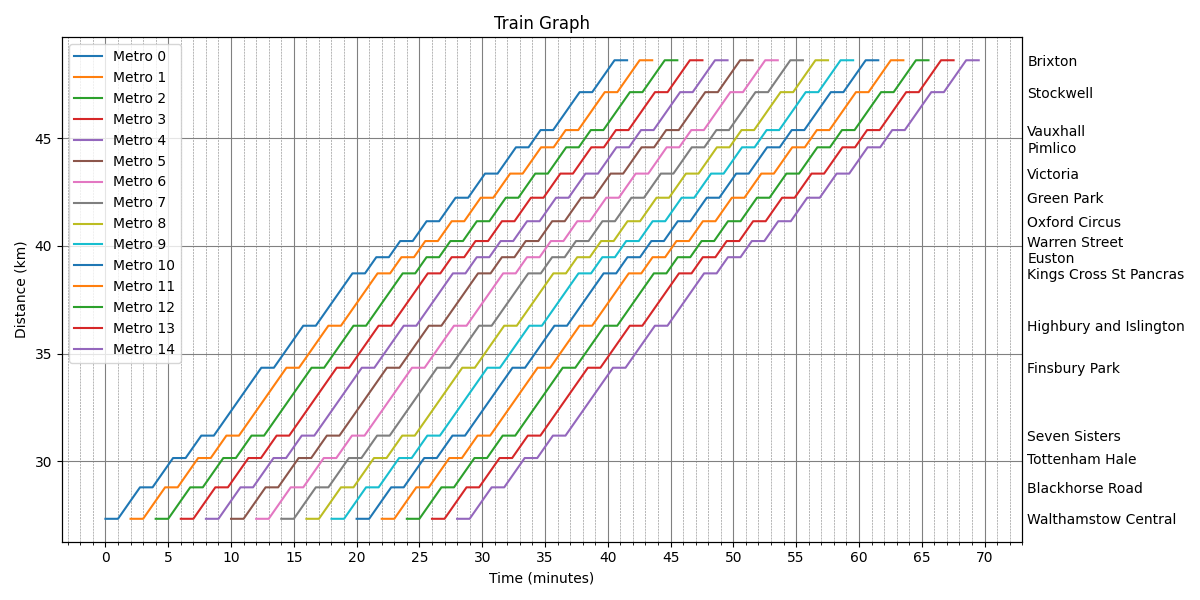
\includegraphics[width=\textwidth]{../train-generator/output/victoria.png}
		\caption{Train graph showing service patterns and station spacing on the Victoria line}
		\label{fig:vic-train-graph}
	\end{figure}
	
	In this activity, you'll take on the role of a timetable planner for a new line. You'll be given details about different services and use a train graph to design a timetable that avoids conflicts and meets operational constraints.
	
	\section{Activity}
	
	You are responsible for planning a timetable for a new single-track railway line. This line runs from station \textbf{A} to station \textbf{G} with intermediate stops at \textbf{B}, \textbf{C}, \textbf{D}, \textbf{E}, and, \textbf{F}. The distance between each station is \qty{5}{\km}, as shown in figure \ref{fig:network-layout}
	
	Each hour, five service must operate on this line:
	\begin{itemize}
		\item Two \textbf{local} trains,
		\item Two \textbf{express} trains, and,
		\item One \textbf{freight} train
	\end{itemize}
	
	\begin{figure}[h]
		\centering
		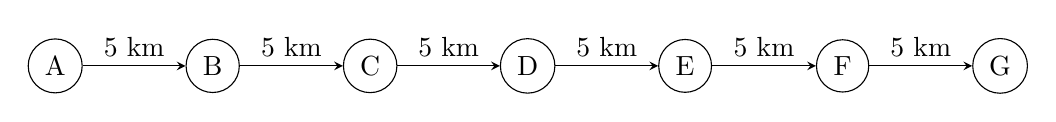
\begin{tikzpicture}[->, >=stealth, node distance=2cm]
			\node[circle, draw] (a) {A};
			\node[circle, draw, right of=a] (b) {B};
			\node[circle, draw, right of=b] (c) {C};
			\node[circle, draw, right of=c] (d) {D};
			\node[circle, draw, right of=d] (e) {E};
			\node[circle, draw, right of=e] (f) {F};
			\node[circle, draw, right of=f] (g) {G};
			
			\draw (a) -- (b) node[midway, above] {5 km};
			\draw (b) -- (c) node[midway, above] {5 km};
			\draw (c) -- (d) node[midway, above] {5 km};
			\draw (d) -- (e) node[midway, above] {5 km};
			\draw (e) -- (f) node[midway, above] {5 km};
			\draw (f) -- (g) node[midway, above] {5 km};
		\end{tikzpicture}
		\caption{Layout and distances for new line}
		\label{fig:network-layout}
	\end{figure}
	
	Details for each service type, including velocity, stopping pattern, and, dwell times are provided in table \ref{tab:services}. Your task is to use this information to create a timetable that fits all five service within a repeatable hourly cycle.
	
	\begin{table}[h]
		\centering
		\caption{Services to run}
		\label{tab:services}
		\begin{tabular}{@{}lllll@{}}
			\toprule
			Train Type & Services per Hour & Max Velocity (\unit{\km \per \hour}) & Intermediate Stops & \Gls{dwell} (\unit{\minute}) \\ \midrule
			Express      & 2                 & 120      & D                  & 2.5                   \\
			Local    & 2                 & 80       & All                & 7                     \\
			Freight    & 1                 & 60       & None               &                       \\ \bottomrule
		\end{tabular}
	\end{table}
	
	Your timetable must satisfy the following constraints:
	\begin{itemize}
		\item All service must depart within \qty{60}{\minute}
		\item The schedule must be designed so that it can be repeated every hour without conflicts.
		\item A minimum \gls{headway} of \qty{5}{\minute} must be maintained between any two trains at any point along the line.
		\item \gls{dwell} must be applied at each scheduled stop.
	\end{itemize}
	
	Use a train graph to plot the movement of each service. The graph should show time on the horizontal axis and distance on the vertical axis. By visualising all five service together, you can identify potential conflicts and adjust departure times, speeds or dwell times to ensure safe and efficient operation.
	
	\section{Extension Tasks}
	If you finish early, here are some extension tasks to explore.
	
	\textbf{Service Spacing}
	
	Try optimising the timetable by spacing similar services evenly through the hour or grouping them closely together. Does this allow more trains per hour? How might it affect passenger experience?
	
	\textbf{Delay simulation} 
	
	Suppose one of the express trains is delayed by \qty{8}{\minute} at station \textbf{D}. What impact does this have on the rest of the timetable? Can you adjust the schedule to recover while still maintaining the minimum headway?
	
	\textbf{Passing Point}
	
	Imagine there is a passing point at station \textbf{D}. How could this be used to improve your timetable? Could it allow for more flexible scheduling or to reduce delays?
	
	\textbf{Turnaround planning}
	
	Consider how trains would turn back at platform \textbf{G} to begin the return service to station \textbf{A}. How many platforms would be needed at stations \textbf{A} and \textbf{G} to support continuous operation? How much turnaround time could be allocated for cleaning or preparation?
	
	\printnoidxglossaries
	
\end{document}